%
\hsection{The Cardinality of Relationships}%
%
\begin{figure}%
%
\subfloat[][%
A 1:1 or one-to-one relationship where participation on both ends is optional. %
An example would be the relation between students and graduation thesis topics.%
\label{fig:relationshipCardinalities:1to1}%
]{\parbox{0.3\linewidth}{\centering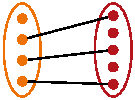
\includegraphics[width=0.85\linewidth]{\currentDir/1to1}}}%
%
\floatSep%
%
\subfloat[][%
A 1:n or 1-to-many relationship where participation on both ends is optional. %
An example would be the relation between supervising professors and students.%
\label{fig:relationshipCardinalities:1ton}%
]{\parbox{0.3\linewidth}{\centering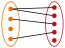
\includegraphics[width=0.85\linewidth]{\currentDir/1ton}}}%
%
\floatSep%
%
\subfloat[][%
A n:m or many-to-many relationship where participation on both ends is optional. %
An example would be the relation between students and course enrollments.%
\label{fig:relationshipCardinalities:ntom}%
]{\parbox{0.3\linewidth}{\centering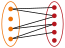
\includegraphics[width=0.85\linewidth]{\currentDir/ntom}}}%
%
\caption{Some somple examples for relationship cardinalities~\cite{SS2005EIDDDFDB:CDDICAMP,V1999C5DMS:CDUTERM}.}%
\label{fig:relationshipCardinalities}%
%
\end{figure}%
%
We already learned that attributes can have different cardinalities:
There can be single-valued or multi-valued attributes and either can be optional.
Similarly, the ends of relationships can have different cardinalities.
In \pgls{UML}, cardinality is called multiplicity.

\Cref{fig:relationshipCardinalities} sketches a set of basic examples for relationship cardinalities.
Commonly, we distinguish one-to-one, one-to-many, and many-to-many relationships.
On a finer granularity level, however, each end of a relationship may have a range of permitted cardinalities.
We distinguish total and partial relationships~\cite{P2006CITRD:ERMI,V1999C5DMS:CDUTERM}.
If all entities of an entity set \emph{must} participate in at least one relationship, then this relationship end \emph{total}.
If only some entities participate in a relationship, then this relationship end is \emph{partial}.

\begin{figure}%
\centering%
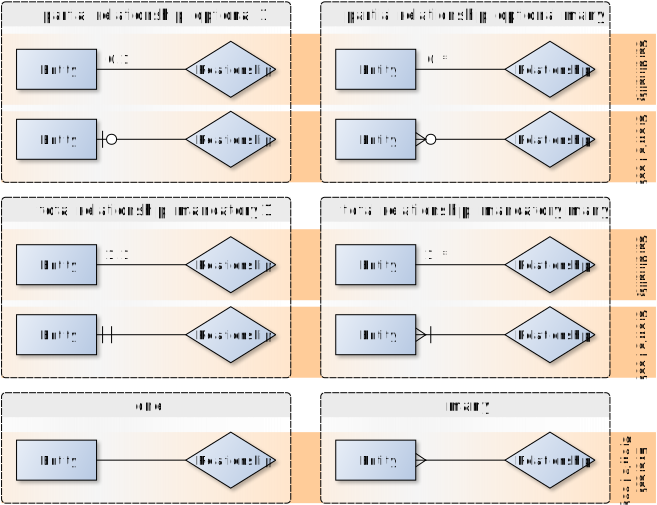
\includegraphics[scale=0.6]{\currentDir/erdCardinalities}%
\caption{Two different ways to express possible cardinalities of relationship ends in \pglspl{ERD}.}%
\label{fig:erdCardinalities}%
\end{figure}%
%
Sadly, there are multiple, sometimes contradicting conventions on how to express the relationship cardinality in an \pgls{ERD}.
On one hand, there is the Crow's Foot notation~\cite{E1976BDSMEWACE,CM2000MDMAUDA,S2024D:CDMERDE}, where a graphical notation expresses the cardinality of a relationship end.
On the other hand, we can also directly write the permitted number of participants as labels on the ends the relationships~\cite{P2006CITRD:ERMI}.
Here, an integer range~\intRange{i}{j}, where $i$~is the minimum number of participating entities, $j$~is the maximum, and $*$~stands for unlimited/many/infinity.
\Cref{fig:erdCardinalities} presents these two methods, along with the original Crow's Foot method by \citeauthor{E1976BDSMEWACE}~\cite{E1976BDSMEWACE}, which did not yet have the mandatory/optional symbolism.

Of course, there are many more possible notations.
In \cite{SS2005EIDDDFDB:CDDICAMP}, we can additionally find a similar notation following the pattern~$(i,j)$ as well as a \citeauthor{C1976TERMTAUVOD}'s original \pgls{ERD} notation~\cite{C1976TERMTAUVOD} where the relationship ends are simply annotated with 1, N, or M to express 1:1, 1:N, or M:N relationships.
Notice that a simple line without any symbol in the Crow's Foot notation stands for \inQuotes{one}~\cite{S2024D:CDMERDE}.
In the arrow-based notation by \citeauthor{B1969DSD}~\cite{B1969DSD}, it stands for \inQuotes{many.}
An arrow touching the relationship diamond means one in~\cite{V1999C5DMS:CDUTERM}.
In~\cite{G2011EW2ITDS:CMUTERM}, the arrow needs to instead touch the entity rectangle and means either~$\geq0$ or~$\geq1$.
This difference probably occurred because \citeauthor{B1969DSD} did not use diamonds for relationships but simply directly connected the entities.
The (min, max) notation is also discussed in~\cite{G2011EW2ITDS:CMUTERM}.

For the remainder of this text, we will stick with Crow's Foot, simply because I can paint this more easily with \yEd\ without needing to add labels to relationship ends.%
%
\FloatBarrier%
\endhsection%
%
